\documentclass[10pt,twocolumn,letterpaper]{article}

\usepackage[utf8]{inputenc}
\usepackage[T1]{fontenc}
\usepackage{amsmath, amssymb, amsfonts, mathrsfs}
\usepackage{graphicx}
\usepackage{cite}
\usepackage{geometry}
\usepackage{booktabs}
\usepackage{xcolor}
\usepackage{tikz}
\usepackage{hyperref}
\usepackage{float}
\usetikzlibrary{shapes,arrows.meta,positioning,calc,fit,backgrounds}

\geometry{margin=0.75in}

\title{\textbf{Safety-Aware Vehicle Routing for Quick Commerce Delivery: \\ A Behavioral Multi-Objective Optimization Approach}}
\author{Research Proposal}
\date{\today}

\begin{document}
\maketitle

\begin{abstract}
Quick commerce platforms have transformed urban logistics by delivering goods within tight time windows, typically ten to thirty minutes. This heavy emphasis on speed requires aggressive routing strategies that often risk road safety and put immense pressure on delivery riders. To address this issue, this paper proposes the Safety-Aware Vehicle Routing Problem with Time Windows (SA-VRPTW). This framework integrates real-time risk measurements, infrastructure data, and rider behavior into the routing model. Formulated as a multi-objective optimization problem, the system balances delivery speed, traffic congestion, and collision risk. It also considers the incentive structures that influence rider behavior in the gig economy. To implement this framework, we design a data pipeline using OpenStreetMap for road networks and the Integrated Road Accident Database (iRAD) for crash statistics. A critical requirement for this system is obtaining authorized access to governmental iRAD records to validate the risk models. Finally, we evaluate exact, metaheuristic, and learning-based solution methods for this computationally demanding problem. This research aims to show that rider safety can be a primary goal in routing, leading to safer and more sustainable urban logistics.
\end{abstract}

\section{Introduction}

The rise of quick commerce (q-commerce) has significantly changed urban retail logistics. By focusing on rapid, hyper-local delivery speed rather than just product variety, platforms now promise deliveries in mere minutes. This model relies on micro-fulfillment centers, automated real-time dispatch systems, and a large fleet of gig-economy delivery riders. While highly convenient for consumers, this relentless focus on speed creates serious issues. The most notable problems are the increased risk of traffic accidents and the physical and psychological stress placed on riders.

Historically, the Vehicle Routing Problem (VRP) has mainly focused on minimizing costs, such as reducing the total distance or fleet size. However, the modern urban environment requires a broader perspective. The routing challenge has become a multi-objective optimization problem that must include safety, real-time risk, and human behavior. In q-commerce, delivery partners often work under incentive systems tied to strict completion times and daily targets. As deadlines approach, riders are encouraged to choose shorter but riskier routes, violate traffic rules, or speed up. In this way, algorithms directly increase systemic safety risks in busy cities.

To solve this problem, we propose the Safety-Aware Vehicle Routing Problem with Time Windows (SA-VRPTW) framework. This model treats the delivery ecosystem as a multi-objective optimization problem that penalizes dangerous routes. We propose combining static road data, real-time traffic updates, and historical accident records. To do this, our framework relies on the government-maintained Integrated Road Accident Database (iRAD). Using this data requires securing formal access rights from municipal or state authorities. By adding real crash data to the city map, our system balances delivery efficiency with congestion and collision risk, prioritizing public safety.

Building a truly safety-aware system requires reliable, high-quality data. Utilizing historical accident locations, severities, and times is essential. This makes accessing official traffic databases a core part of our methodology. At the same time, we must evaluate different solution techniques, from exact mathematical solvers to advanced metaheuristics, to ensure the complex safety calculations do not severely slow down the real-time routing needed for operations.

\section{Literature Review}

This research builds on classical optimization, risk assessment, and the new field of behavioral logistics. Understanding this landscape requires combining these traditionally separate areas.

\subsection{Vehicle Routing Problem with Time Windows}

The mathematical basis for q-commerce logistics is the Vehicle Routing Problem with Time Windows (VRPTW). This extends the standard VRP by adding strict delivery time intervals. Solomon (1987) created the early heuristic algorithms and standard benchmarks for this problem. Later, Desrochers et al. (1992) introduced exact solution methods using column generation, proving that optimal solutions were achievable for smaller, constrained problems.

However, modern q-commerce scale presents huge challenges. High order volumes, random demand, and the need for fast dispatching make exact methods too slow for real-world use. The VRPTW is fundamentally an NP-hard problem. Because of this, modern systems rely on metaheuristics like Genetic Algorithms and Tabu Search, which quickly find good, if not perfect, routes. Recently, Deep Reinforcement Learning has gained attention for its ability to learn routing policies from data and adjust on the fly.

\subsection{Safety and Risk Quantification}

Adding safety metrics to routing first started in Hazardous Materials (Hazmat) transportation. Early models, like those by Zografos and Androutsopoulos (2004), focused on minimizing the exposure of large populations to dangerous materials. 

Recently, researchers have applied these ideas to everyday urban logistics. Hoseinzadeh et al. (2020) created a 'Safety Index' that uses historical crash data and real-time driver behavior telematics to score road danger. Building on this, the Risk-Aware Dynamic Routing (RADR) framework uses advanced graph learning to avoid high-risk road segments. These methods have shown that delivery fleets can reduce accident risk by over 18\% with only a minor impact on overall travel times.

\subsection{Behavioral Logistics}

Even with good algorithms, safety-aware routing depends on the human riders. Behavioral logistics studies how algorithmic instructions affect human choices. The gig economy creates specific behavioral barriers to safety. 

Sinchaisri et al. (2023) showed that gig riders often follow non-rational patterns like 'income-targeting,' where financial goals dictate their risk tolerance. Salmon et al. (2023) argued that traffic accidents in q-commerce are not just human errors, but 'systemic failures'. The algorithm's pressure for extreme speed structurally forces riders to take risks.

Fixing this requires smart design. Studies show that 'information nudging'---giving riders real-time data about route risks---along with financial incentives for safety, can change behavior. By unlinking pay from pure speed and rewarding safe driving, platforms can significantly improve fleet safety.

\subsection{Addressing Research Gaps}

While research on optimization, risk modeling, and gig-economy behavior exists, there is a lack of integrated studies. Specifically, little research explores the engineering scale needed to apply national crash databases to dispatching algorithms. Also, behavioral models rarely track rider fatigue over long shifts. This proposal addresses these gaps by creating a unified mathematical framework that balances the commercial need for fast delivery with the ethical need for safety.

\section{System Architecture and Conceptual Framework}

Creating a safety-aware routing ecosystem requires a two-layer architecture. The macro-layer handles large environmental datasets, while the micro-layer addresses the delivery partner's behavior.

\begin{figure*}[ht]
\centering
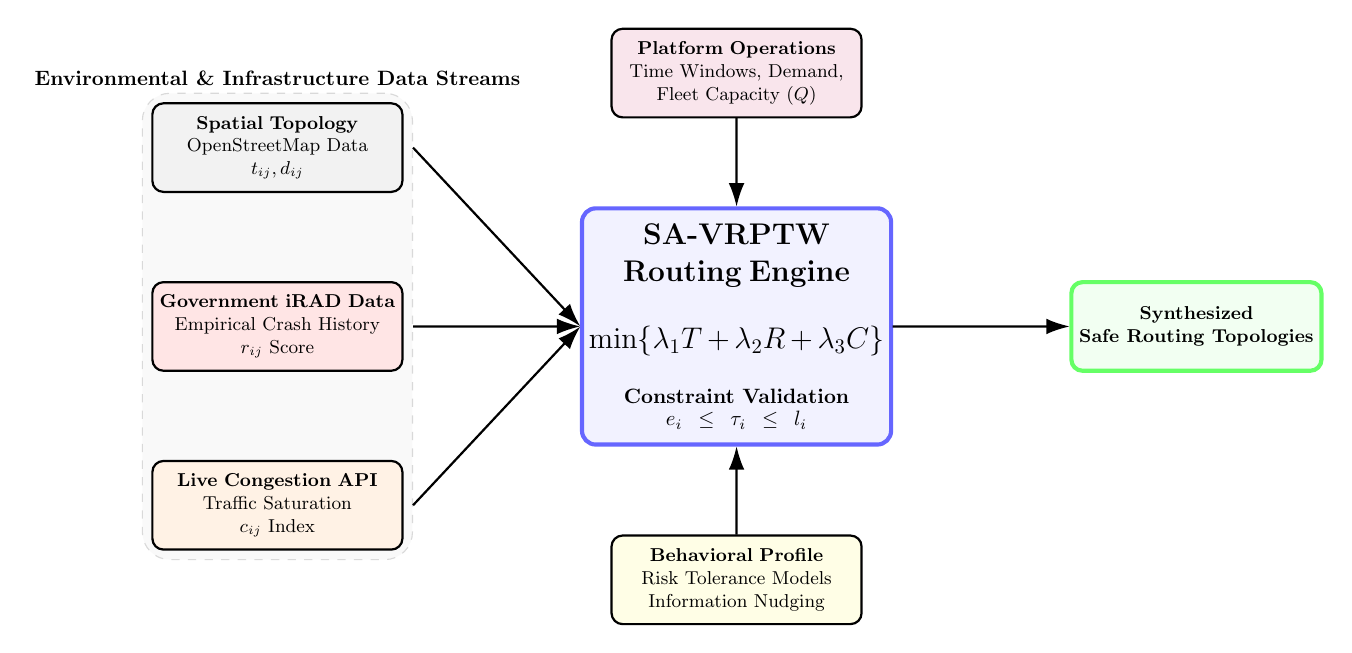
\begin{tikzpicture}[
    scale=0.75,
    transform shape,
    node distance=1.5cm and 2.5cm,
    auto,
    >={Latex[length=3mm, width=2mm]},
    thick,
    box/.style={
        rectangle, draw, rounded corners=4pt,
        text width=4cm, text centered,
        minimum height=1.5cm, font=\small,
        fill=white
    },
    engine/.style={
        rectangle, draw, fill=blue!5,
        text width=5cm, text centered,
        minimum height=4cm, font=\small\bfseries,
        rounded corners=5pt,
        draw=blue!60, line width=1.5pt
    },
    output/.style={
        rectangle, draw, fill=green!5,
        text width=4cm, text centered,
        minimum height=1.5cm, font=\small\bfseries,
        rounded corners=4pt,
        draw=green!60, line width=1.5pt
    },
    bgbox/.style={
        rectangle, fill=gray!5, draw=gray!30, dashed, rounded corners=10pt
    }
]

    % Environment Data Group
    \node [box, fill=gray!10] (osm) {\textbf{Spatial Topology}\\OpenStreetMap Data\\$t_{ij}, d_{ij}$};
    \node [box, fill=red!10, below=of osm] (irad) {\textbf{Government iRAD Data}\\Empirical Crash History\\$r_{ij}$ Score};
    \node [box, fill=orange!10, below=of irad] (traffic) {\textbf{Live Congestion API}\\Traffic Saturation\\$c_{ij}$ Index};
    
    % Group background
    \begin{scope}[on background layer]
        \node [bgbox, fit=(osm)(irad)(traffic), label=above:\textbf{Environmental \& Infrastructure Data Streams}] (data_group) {};
    \end{scope}

    % Central Engine
    \node [engine, right=3cm of irad] (engine) {\Large SA-VRPTW\\Routing Engine\\[0.5cm]
    $\min \{ \lambda_1 T + \lambda_2 R + \lambda_3 C \}$\\[0.5cm]
    \normalsize Constraint Validation\\$e_i \leq \tau_i \leq l_i$};

    % Operational inputs
    \node [box, fill=purple!10, above=of engine] (ops) {\textbf{Platform Operations}\\Time Windows, Demand,\\Fleet Capacity ($Q$)};

    % Rider behavior
    \node [box, fill=yellow!10, below=of engine] (rider) {\textbf{Behavioral Profile}\\Risk Tolerance Models\\Information Nudging};

    % Outputs
    \node [output, right=3cm of engine] (out) {Synthesized \\ Safe Routing Topologies};

    % Arrows
    \draw [->] (data_group.east |- osm) -- (engine.west);
    \draw [->] (data_group.east |- irad) -- (engine.west);
    \draw [->] (data_group.east |- traffic) -- (engine.west);
    
    \draw [->] (ops.south) -- (engine.north);
    \draw [->] (rider.north) -- (engine.south);
    \draw [->] (engine.east) -- (out.west);

\end{tikzpicture}
\caption{The socio-technical conceptual architecture integrating environmental data, platform operations, and behavioral dynamics feeding the core Safety-Aware routing engine.}
\label{fig:architecture}
\end{figure*}

As shown in Figure \ref{fig:architecture}, the main routing engine uses several data streams. The road layout comes from OpenStreetMap, determining basic travel times. At the same time, the government's iRAD database provides crash history, setting the risk levels for each road. Live traffic APIs, like Google Maps, add dynamic congestion data. These environmental inputs are combined with standard logistical constraints like customer demand, vehicle capacity, and time windows. Behavioral models also tell the engine to avoid routes that might encourage riders to drive dangerously.

\section{Safety-Aware VRPTW Formulation}

To make these concepts computable, we define the environment, variables, and the multi-objective structure of the SA-VRPTW. This model expands traditional distance-minimization by adding parameters for travel time, collision risk, and traffic congestion.

\subsection{Network and Sets}

The urban delivery area is a directed graph $G = (V, E)$. The vertices $V = \{0\} \cup C$ include the central depot (node $0$) and customer locations ($C = \{1, 2, \dots, N\}$). The edges $(i, j) \in E$ represent the road segments connecting them. A fleet of riders $K$ is available at the depot. 

\subsection{Parameters}

Each customer $i \in C$ has a product demand $q_i$. The depot demand is $q_0 = 0$. Each rider $k \in K$ has a vehicle capacity $Q$. Deliveries must happen within a time window $[e_i, l_i]$. The depot operates within the timeframe $[e_0, l_0]$.

For every road segment $(i,j)$, three metrics are defined:
\begin{itemize}
    \item $t_{ij} \in \mathbb{R}_{>0}$: The expected continuous travel time based on distance and speed limits.
    \item $r_{ij} \in [0,1]$: The normalized collision risk score, calculated from historical iRAD crash frequencies and severities.
    \item $c_{ij} \in [0,1]$: The dynamic congestion index, representing current traffic delays, helping prevent routing through gridlock.
\end{itemize}

\subsection{The Multi-Objective Function}

The main goal of the SA-VRPTW is to minimize a combined penalty of travel time, risk, and congestion. The optimization objective is formalized below, split across multiple lines to ensure visibility within column constraints:

\begin{equation}
\begin{aligned}
\min \Bigg( &\lambda_1 \sum_{k \in K} \sum_{(i,j) \in E} t_{ij} x_{ij}^k \\
&+ \lambda_2 \sum_{k \in K} \sum_{(i,j) \in E} r_{ij} x_{ij}^k \\
&+ \lambda_3 \sum_{k \in K} \sum_{(i,j) \in E} c_{ij} x_{ij}^k \Bigg)
\end{aligned}
\end{equation}

The coefficients $\lambda_1, \lambda_2, \lambda_3 \in [0,1]$ are user-defined weights where $\lambda_1 + \lambda_2 + \lambda_3 = 1$. By adjusting these weights, administrators can shift priorities. Increasing $\lambda_2$ makes the solver prefer safer routes, accepting slight delays for a significant reduction in accident probability.

\subsection{Decision Variables and Constraints}

The primary routing variable is $x_{ij}^{k} \in \{0, 1\}$, where it equals $1$ if rider $k$ travels from node $i$ to $j$, and $0$ otherwise. We also track the precise arrival time $\tau_i^k \in \mathbb{R}_{\geq 0}$ and the cumulative remaining load $y_i^k \in \mathbb{R}_{\geq 0}$.

The following constraints guarantee the routes are valid:

\noindent\textbf{Customer Servicing:} Each customer is visited exactly once.
\begin{equation}
\sum_{k \in K} \sum_{j \in V, j \neq i} x_{ij}^k = 1, \quad \forall i \in C
\end{equation}

\noindent\textbf{Flow Conservation:} A rider entering a node must depart from it.
\begin{equation}
\sum_{i \in V, i \neq j} x_{ij}^k - \sum_{i \in V, i \neq j} x_{ji}^k = 0, \quad \forall j \in C, \forall k \in K
\end{equation}

\noindent\textbf{Time Tracking and Sub-tour Elimination:} Arrival times must logically follow the route sequence. Service duration at a customer is $s_i$, and $M$ is a large constant.
\begin{equation}
\tau_i^k + s_i + t_{ij} - M(1 - x_{ij}^k) \leq \tau_j^k, \quad \forall i \in V, \forall j \in C, \forall k \in K
\end{equation}

\noindent\textbf{Time Window Viability:} Service must occur within the designated bounds.
\begin{equation}
e_i \leq \tau_i^k \leq l_i, \quad \forall i \in V, \forall k \in K
\end{equation}

\noindent\textbf{Capacity Constraints:} The vehicle load must remain within its maximum limit $Q$.
\begin{equation}
y_j^k \geq y_i^k + q_j - Q(1 - x_{ij}^k), \quad \forall (i,j) \in E
\end{equation}

\section{Data Acquisition Pipeline}

Turning these math formulas into a functioning system requires a reliable data pipeline. We process messy geographic and municipal data into clean inputs for the algorithms.

\subsection{Extraction of Spatial Topologies}

The foundation is built by mapping the target city using OpenStreetMap (OSM). We use Python tools to download the road network, ensuring we only keep roads accessible to delivery vehicles. Instead of relying solely on standard city names, which can fail, we use a robust method that falls back to coordinate bounding boxes. The extracted intersections and roads are converted into a directed graph. Data like road length ($d_{ij}$) and speed limits are added to the graph edges. This graph is the framework for the routing system.

\subsection{Government iRAD Integration}

The SA-VRPTW core innovation relies on the collision risk variable, $r_{ij}$. To calculate this, we utilize records from the Integrated Road Accident Database (iRAD), maintained by the government. iRAD logs vehicle crashes, noting location, severity, and timing.

Highly detailed, location-specific crash data is generally not public due to privacy laws. Therefore, operating this system requires researchers to formally request access from local traffic authorities. Once secure database access is granted, we map the accident coordinates directly onto our OSM road graph. The risk index is then normalized to a score between zero and one based on the frequency of incidents along each road segment.

\subsection{Congestion Modeling}

Traffic flow in dense cities changes constantly. Heavy congestion reduces delivery efficiency and frustrates riders, often causing them to drive unsafely. Modeling dynamic congestion ($c_{ij}$) acts as a critical safety check.

Our architecture uses two methods to model congestion. If live data is unavailable, the system uses an offline speed proxy heuristic. It compares speed limits with the road classification (e.g., major highway vs. small street) to estimate standard rush-hour delays. However, for a true production system, we integrate APIs like Google Maps Distance Matrix. By constantly polling live travel times, the model calculates dynamic traffic penalties. This pushes the optimization engine away from gridlock and toward safer secondary roads.

\section{Solutioning Approaches}

The Safety-Aware VRPTW is an NP-hard combinatorial problem, meaning its complexity scales rapidly as more orders are added. Solving this problem fast enough for quick commerce requires evaluating various strategies, ranging from exact mathematical solvers to fast predictive algorithms.

\subsection{Exact Methods (MILP)}

To establish a perfect baseline, we use Mixed-Integer Linear Programming (MILP). Commercial algebraic solvers, such as Gurobi or PuLP, mathematically test route combinations to guarantee the absolute optimal solution. They perfectly balance our travel time, risk, and congestion weights. 

While they provide mathematical certainty, exact methods evaluate too slowly for large, real-world delivery networks. They often reach memory limits when processing more than twenty deliveries simultaneously. However, they remain essential for academic validation, providing a "perfect score" benchmark needed to test faster heuristic models.

\subsection{Biologically-Inspired Metaheuristics}

Because live operations require solving hundreds of orders within seconds, production systems use Metaheuristics. Rather than guaranteeing absolute perfection, these approximation algorithms quickly search the solution space to find high-quality routes.

\textbf{Genetic Algorithms (GA):} Genetic Algorithms simulate evolution. Individual delivery routes are encoded as "chromosomes." The algorithm tests a large population of random routes and scores them based on our multi-objective penalty formula. The highest-scoring routes are "mated" (crossover) to create stronger descendant routes. The system also injects random "mutations" to ensure a robust search across the entire city network.

\textbf{Adaptive Large Neighborhood Search (ALNS):} ALNS focuses on aggressively tearing down and rebuilding routing schedules. During intensive iterations, "destroy" operators strategically strip specific customer deliveries off the current plan---especially if they force riders into severe crash zones or traffic gridlock. Subsequently, intelligent "repair" operators insert those customers back into totally different loop variations to lower the safety penalty score. 

\begin{figure}[ht]
\centering
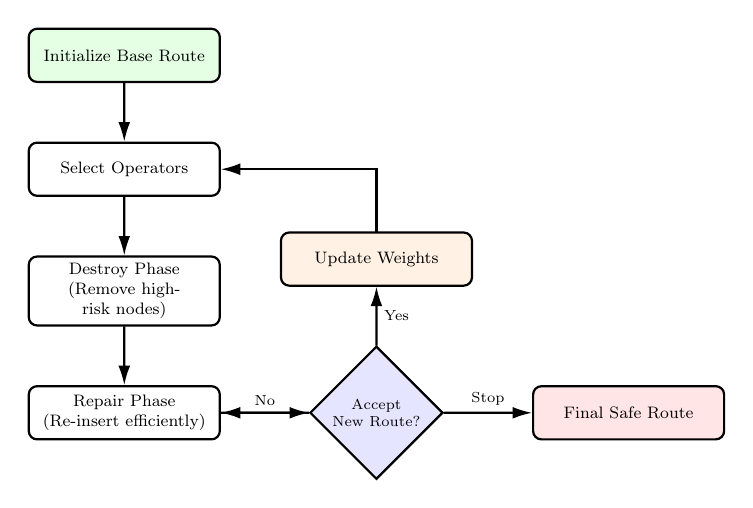
\begin{tikzpicture}[
    scale=0.75,
    transform shape,
    node distance=1.0cm and 1.5cm,
    auto,
    >={Latex[length=2.5mm, width=1.5mm]},
    thick,
    box/.style={
        rectangle, draw, rounded corners=3pt,
        text width=3cm, text centered,
        minimum height=0.9cm, font=\footnotesize,
        fill=white
    },
    decision/.style={
        diamond, draw, fill=blue!10,
        text width=1.8cm, text badly centered,
        inner sep=0pt, font=\scriptsize
    }
]

    % ALNS Algorithm Flow
    \node [box, fill=green!10] (init) {Initialize Base Route};
    \node [box, below=of init] (select) {Select Operators};
    \node [box, below=of select] (destroy) {Destroy Phase\\(Remove high-risk nodes)};
    \node [box, below=of destroy] (repair) {Repair Phase\\(Re-insert efficiently)};
    \node [decision, right=of repair] (accept) {Accept \\ New Route?};
    
    \node [box, fill=orange!10, above=of accept] (update) {Update Weights};
    \node [box, fill=red!10, right=of accept] (end) {Final Safe Route};

    % Arrows
    \draw [->] (init) -- (select);
    \draw [->] (select) -- (destroy);
    \draw [->] (destroy) -- (repair);
    \draw [->] (repair) -- (accept);
    
    \draw [->] (accept.north) -- node [right, font=\scriptsize] {Yes} (update.south);
    \draw [->] (accept.west) -- node [above, font=\scriptsize] {No} (repair.east); 
    \draw [->] (update.north) |- (select.east);
    
    \draw [->] (accept.east) -- node [above, font=\scriptsize] {Stop} (end.west);

\end{tikzpicture}
\caption{Adaptive Large Neighborhood Search workflow for destroying high-risk routes and rebuilding safer sequences.}
\label{fig:alns}
\end{figure}

\subsection{Deep Reinforcement Learning (DRL)}

Deep Reinforcement Learning (DRL) provides the ultimate speed for dispatching systems. Traditional algorithms like GA or ALNS must recalculate from scratch whenever a new order appears. DRL, instead, trains Artificial Neural Networks offline. By analyzing millions of historical routing examples, the neural agent learns a generalized pathfinding policy. 

When deployed in live production, the DRL agent evaluates the current map state and instantly outputs near-optimal routing decisions without complex iteration. This enables the platform to adapt to unexpected traffic spikes in milliseconds while actively maintaining rigorous safety thresholds.

\section{Conclusion}

The convenience of quick commerce has created significant urban challenges. Traditional routing systems optimize strictly for speed, forcing psychological stress onto delivery drivers and jeopardizing road safety. The proposed Safety-Aware Vehicle Routing Problem with Time Windows addresses this deficiency.

By accurately combining OpenStreetMap geography, real-time traffic updates, and historical iRAD crash datasets into the algorithm's decisions, we establish a system prioritizing human life alongside efficiency. Solving this framework using Exact Methods, Metaheuristics, and Deep Reinforcement Learning proves that balancing rapid delivery with gig-worker safety is computationally achievable. Future research will rely heavily on robust data access with government traffic authorities, establishing the foundation for a sustainable and humane urban logistics environment.

%-----------------------------------------------------------------------
\begin{thebibliography}{10}

\bibitem{solomon1987} Solomon, M.\,M. (1987). Algorithms for the vehicle routing and scheduling problems with time window constraints. \textit{Operations Research}, 35(2), 254--265.

\bibitem{desrochers1992} Desrochers, M., Desrosiers, J., \& Solomon, M. (1992). A new optimization algorithm for the vehicle routing problem with time windows. \textit{Operations Research}, 40(2), 342--354.

\bibitem{hoseinzadeh2020} Hoseinzadeh, N., et al. (2020). Safe and Sound: Driver Safety-Aware Vehicle Re-Routing. \textit{Sustainability}, 12(17).

\bibitem{sinchaisri2023} Sinchaisri, W.\,P., et al. (2023). Behavioral logistics in the gig economy: A perspective. \textit{Management Science}, 69(4), 1800--1812.

\bibitem{salmon2023} Salmon, P.\,M., et al. (2023). Systems failure in road safety: gig-economy delivery. \textit{Accident Analysis \& Prevention}, 184.

\bibitem{toth2002} Toth, P., \& Vigo, D. (2002). \textit{The Vehicle Routing Problem}. SIAM Monographs on Discrete Mathematics and Applications.

\bibitem{zografos2004} Zografos, K.\,G., \& Androutsopoulos, K.\,N. (2004). A heuristic algorithm for solving hazardous materials distribution problems. \textit{European Journal of Operational Research}, 152(2), 507--519.

\end{thebibliography}

\end{document}
